\documentclass[12pt, journal, compsoc]{IEEEtran}
\usepackage[utf8]{inputenc}
\usepackage{verbatim}
\usepackage{graphicx}
\usepackage{caption}
\usepackage{cprotect}
\usepackage{mathtools}

\title{\LaTeX\ Tutorial}

\author{Shayan Bathaee}

\date{October 2021}
\begin{document}

\markboth{\LaTeX\ IEEE Template Tutorial}{}

\IEEEcompsoctitleabstractindextext{
\begin{abstract}
    This is a tutorial for creating a \LaTeX\ document in IEEE format. It will cover all the basic necessities for making a document like this one. Topics included will be creating a \LaTeX\ file, sections, subsections, body text, tables, images, mathematical formulas, acknowlegements, and citations. 
\end{abstract}

\begin{IEEEkeywords}
    CSE185, \LaTeX\ Tutorial, IEEEtran, \LaTeX, Document, Template
\end{IEEEkeywords}}

\maketitle

\section{Introduction}
If you're reading this, you probably want to know how to write a \LaTeX\ document. Well, you've come to the right place. If you can make it to the end of this document, you should come out with a decent grasp of creating a \LaTeX\ document from beginning to end.

\vspace{12pt}

\noindent \textbf{Why will this tutorial be helpful?}

\noindent In this tutorial, you will learn how to...
\begin{itemize}
    \item Create a \LaTeX\ file
    \item Make sections and subsections
    \item Write body text
    \item Create tables
    \item Display images
    \item Write mathematical formulas
    \item Make an acknowledgements section
    \item Make a citations section
\end{itemize}

\vspace{12pt}

\noindent \textbf{Why should you learn \LaTeX?}

\noindent \LaTeX\ is an incredibly useful tool for designing documents. There is a wide range of resources that make it possible for you to display any type of text you want. As an engineering student, it makes it especially easy for me to create mathematical equations, display diagrams, and make my homework look neat. No matter who you are or why you want to learn \LaTeX, there is certainly going to be something in here that will interest you.

\section{Creating a \LaTeX\ Document}
In this section, you will learn how to make a \LaTeX\ document. We will go through all the basics you need to get started.
\subsection{Environments}
In \LaTeX, much of your work is done within an environment. In fact, one of the first steps to creating a document is setting up an environment. Environments simply format blocks of code in \LaTeX\ \cite{overleaf:environments}. Environments start with a \verb|\begin{}| and end with a \verb|\end{}|. What you put inside the brackets dictates what environment you will be in.

\vspace{12pt}

\noindent For example, if I wrote \verb|\begin{document}|, I would be inside of my \LaTeX\ document. Anything I typed would affect what my document looks like. After I am finished in my document, I would simply write the line \verb|\end{document}| to exit the environment. As we will see later, environments are used for much more than just beginning and ending documents. 

\subsection{Reserved Characters}
In \LaTeX, there are some characters that have special functions \cite{latexref:reserved}. Because of this, you may have to use some commands to get them into your normal text. Let's go through each of the reserved characters and what they do.

\begin{enumerate}
    \item The "\verb|\|" character is used to indicate a new command.
    \item The "\verb|~|" character is used to indicate an unbreakable space. It essentially makes sure the word before it and the word after are placed on the same line.
    \item The "\verb|\\|" character is used to indicate a new line.
    \item The "\verb|%|" character is used to indicate a comment in the source code.
\end{enumerate}
You are probably wondering: What if I want to display one of those characters in normal~text? The answer is quite easy. Most of the time, you can get away with just putting a backslash in front of the reserved character you want to use. For example, typing \verb|\%| would result in \%. If you wanted to type a backslash, you would have to write \verb|\textbackslash| which would result in \textbackslash. Of course, you could type it twice to get the new line character: \textbackslash\textbackslash.

\subsection{Preamble}
The preamble in a \LaTeX\ file is the source code that comes before the document begins \cite{overleaf:preamble}. The preamble begins with the command \verb|\documentclass[]{}|. Using this command, you can set the font size, document type, page size, and more. For example, the command \verb|\documentclass[12pt]{article}| would set up the document to be structured as an article, having a base font size of 12.

\vspace{12pt}

\noindent Another part of the preamble is using packages. Packages in \LaTeX\ give you more abilities than you would normally have. They will allow you do do things such as write complex math, change the styling of your document, and lots more. To use a package, simple type the command \verb|\usepackage{}| with the package name in brackets. You can also change options in packages by doing \verb|\usepackage[options]{package}|.

\vspace{12pt}

\noindent For example, at the start of this document I included the command \verb|\usepackage{verbatim}|. This package allows me to put code in my document. Using the package, if I typed \verb!\verb|\LaTeX\|!, it would display \verb|\LaTeX\|.

\subsection{Title and Heading Information}
The last basic things that you'll want to include in your preamble is the title, the authors name, and the date. To make the title, write the command \verb|\title{your title}|. To write the author's name, simply type \verb|\author{author's name}|. To set the~date, write \verb|\date{the date}|.

\vspace{12pt}

\noindent Typing the command \verb|\maketitle| will create the title on it's own title page. However, in some document classes it will only put the title at the top-center of the first page \cite{nasa}.

\section{Sections}
Now that you know how to set up a basic \LaTeX\ document, we can move on to the document content. The first thing we'll start with is sections and subsections. 

\vspace{12pt}

\noindent This document is broken down into sections. The sections we have looked at so far were the Introduction, and Creating a \LaTeX\ Document. Sections can be made quite easily. All you have to do is type the command \verb|\section{section name}|.

\subsection{Subsections}
You may have also noticed that this document has subsections. For example, the Environments section is a subsection of the Creating a \LaTeX\ Document section. To make a subsection, you can simply type in the command \verb|\subsection{subsection name}|. In~fact, you can take it one step further by writing the command \verb|\subsubsection{}| to create a nested subsection.

\section{Body Text}
For the most part, when you are writing body text you can just type like normal. Occasionally though, you may want to spice up your paragraphs a little bit. Because most of these operations are fairly easy, I decided to include a list of operations you can do to make your body text a little bit nicer \cite{overleaf:fonts}.
\begin{itemize}
    \item \verb|\textbf{}| - \textbf{Bold text}
    \item \verb|\underline{}| - \underline{Underline text}
    \item \verb|\textit{}| - \textit{Italicize text}
    \item \verb|\small{}| - \small{Small text}\normalsize
    \item \verb|\tiny{}| - \tiny{Tiny text}\normalsize
    \item \verb|\large{}| - \large{Large text}\normalsize
    \item \verb|\huge{}| - \huge{Huge text}\normalsize
    \item \verb|\normalsize{}| - \normalsize{Normal text}
    \item \verb|\texttt{}| - \texttt{Typewriter text}
    \item \verb|\textsf{}| - \textsf{Sans Serif text}
    \item \verb|\textsc{}| - \textsc{Small Caps text}
    \item \verb|\textsl{}| - \textsl{Slanted text}
    \item \verb|\LaTeX\ | - \LaTeX\ 
\end{itemize}

\section{Tables}
Making a table can be slightly challenging at first. The first step you'll want to do is center your table using the command \verb|\begin{center}| \cite{overleaf:tabular}. Now, you can begin constructing the table. Let's make a simple 2x4 table. You will need to start with the command \verb|\begin{tabular}| (not to be confused with \verb|\begin{table}|, which is a float table environment that allows for more positioning options). This is followed by a declaration of how many columns you want (two in our case) which will be formatted as \verb|{c c}|.

\vspace{12pt}

\noindent Now that we have set up the size of our table, we can set the elements in each row. To set the elements of a row, we write \verb|item1 & item2 \\|, using the double backslash to indicate a new row. Once we have set up all of the rows, we can end the tabular environment and the center environment. All together, our source code should look like this:
\begin{verbatim}
\begin{center}
    \begin{tabular}{c c}
        item1 & item2 \\
        item3 & item4 \\
        item5 & item6 \\
        item7 & item8 \\
    \end{tabular}
\end{center}
\end{verbatim}
Resulting in this table:
\vspace{12pt}
\begin{center}
    \begin{tabular}{c c}
        item1 & item2 \\
        item3 & item4 \\
        item5 & item6 \\
        item7 & item8 \\
    \end{tabular}
\end{center}
\vspace{12pt}
Adding a \texttt{|} into the column declaration will add vertical boundaries to the table, and we can add as many as we want. Adding a \verb|\hline| before a row will insert a horizontal line. For example, take this new code:
\begin{verbatim}
\begin{center}
    \begin{tabular}{||c|c|}
        \hline\hline
        item1 & item2 \\
        \hline
        item3 & item4 \\
        \hline
        item5 & item6 \\
        item7 & item8 \\
        \hline
    \end{tabular}
\end{center}
\end{verbatim}
And look at the result:
\vspace{12pt}
\begin{center}
    \begin{tabular}{||c|c|}
        \hline\hline
        item1 & item2 \\
        \hline
        item3 & item4 \\
        \hline
        item5 & item6 \\
        item7 & item8 \\
        \hline\hline
    \end{tabular}
\end{center}
\vspace{12pt}
Take a look at how the table has double lines, single lines, and no lines in some places. The whole table is completely configurable.

\vspace{12pt}

\noindent If you wanted to left align the left column and right align the right column, there's an easy way to do that too. Instead of configuring the columns with the letter '\verb|c|', instead use an '\verb|l|' for left alignment and a '\verb|r|' for right alignment. Let's look at an example:
\begin{verbatim}
\begin{center}
    \begin{tabular}{|l|r|}
        \hline
        hi & hello \\
        \hline
        hello & hi \\
        \hline
    \end{tabular}
\end{center}
\end{verbatim}
This code will result in the following table:
\vspace{12pt}
\begin{center}
    \begin{tabular}{|l|r|}
        \hline
        hi & hello \\
        \hline
        hello & hi \\
        \hline
    \end{tabular}
\end{center}
\vspace{12pt}


\noindent As you can see, the left column is now left aligned and the right column is right aligned. This is just scratching the surface of what's possible with tables, especially considering the packages available for creating even more complex ones.

\section{Figures}
Say I wanted to show you an image of a banana slug, along with a small description of the image below it. How would I do such a thing? The first step would be to go all the way back to the preamble \cite{wikibooks:figures}. We are going to need to add a package using the following command: \verb|\usepackage{graphicx}|. Once we have the graphicx package, we can run the command \verb|includegraphics{file name}| (if you are using offline tools for \LaTeX, you may need to specify the file location using \verb|\graphicspath{file path}| in your preamble).

\vspace{12pt}

\noindent When you display the graphic, it may look pretty bad. This is likely because you need to adjust the size parameters. You can do so by running the command in the following way: \verb|\includegraphics[scale=_]{file}|. There are other parameters besides \texttt{scale} that you can use, such as adjusting the width, height, angle, etc.

\vspace{12pt}

\noindent Let's try displaying the image of my slug now. For my purposes, I'm going to make the image scaled down by 1/8 using the scale parameter. I'm also going to center the image using the \verb|\begin{center}| environment that we used earlier.

\vspace{12pt}

\begin{center}
    
\includegraphics[scale = 0.125]{slug.pdf}
\end{center}

\vspace{12pt}

\noindent The last step to adding an image is creating a caption. To start, we will want to use the \verb|\usepackage{caption}| command in our preamble. Next, we would have to use the \verb|figure| environment. For this example, I'm going to use a Titration plot. The code will look like this:
\footnotesize
\begin{verbatim}
\begin{figure}[h]
    \centering
    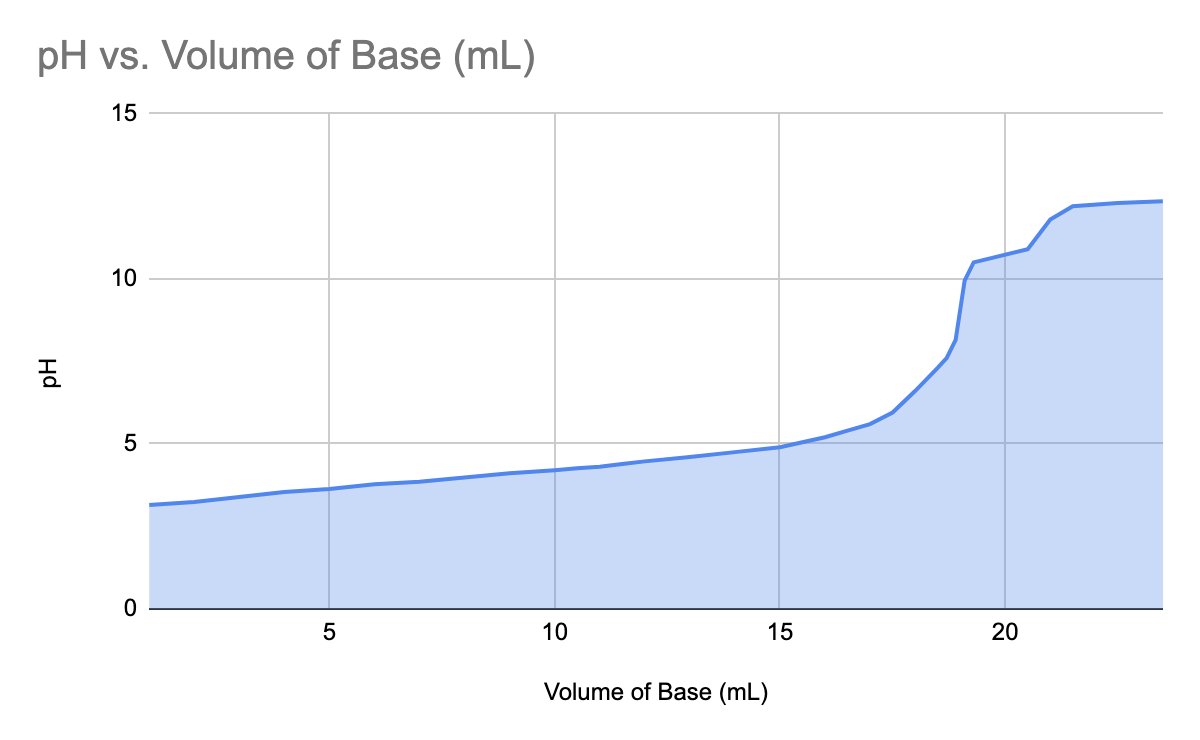
\includegraphics[scale=0.4]{titration.png}
    \caption{This is a Titration plot...}
\end{figure}
\end{verbatim}
\normalsize
Let's break this down line by line. We start by beginning a new figure, with the parameter \verb|[h]|. The \verb|[h]| tells \LaTeX\ to place the image approximately where it appears in the source code. Next, we center the image, call the \verb|\includegraphics| command, center and set set the caption. Once all of that is done, we can end the figure and display it:
\begin{figure}[h]
    \centering
    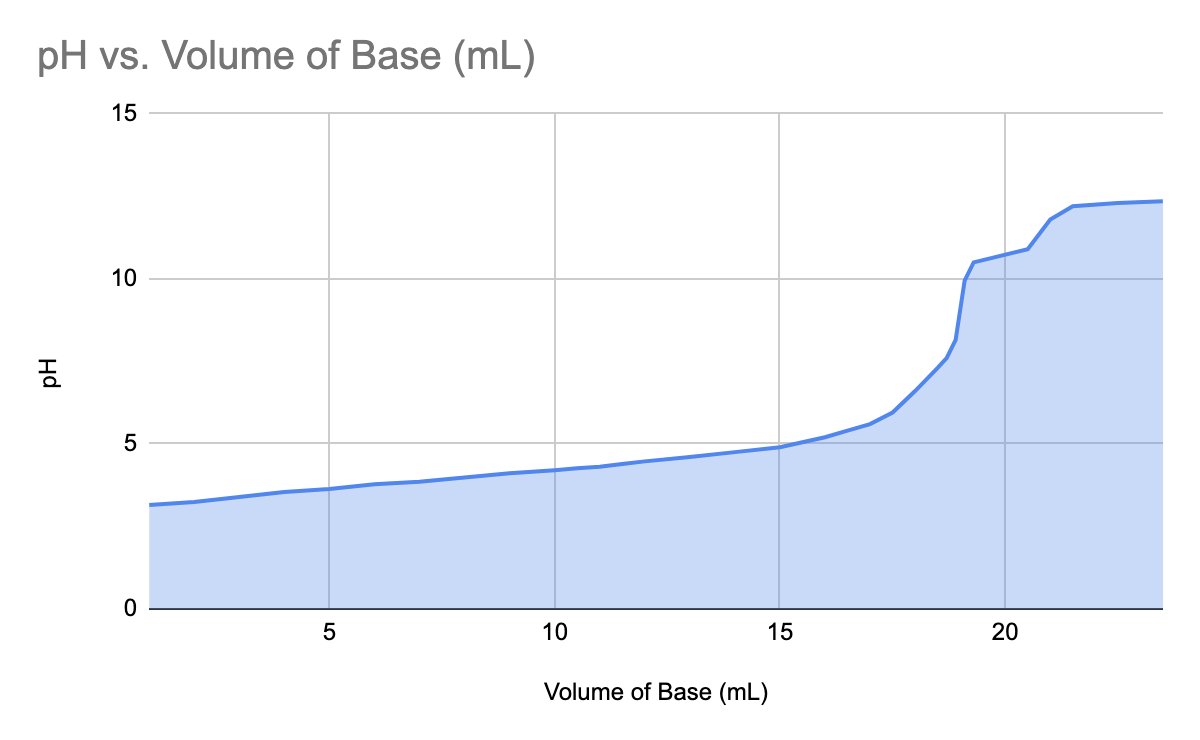
\includegraphics[scale=0.4]{titration.png}
    \captionsetup{justification=centering}
    \caption{This is a Titration plot. I created this Titration plot in google spreadsheets by entering data into the cells and plotting it.}
\end{figure}

\section{Mathematical Formulas}
\label{math}
In this section, we are going to be learning about one of the most useful parts of \LaTeX. In \LaTeX, it is extraordinarily easy to make very beautiful mathematical equations. This makes it perfect for typing up math homework, writing proofs, and much more. Let's get started exploring a few of the many mathematical tools in \LaTeX.

\subsection{Equation Environments}
When writing mathematical equations in \LaTeX, there are two possible environments to work with. There is an inline environment, and a display environment \cite{doc2latex}. The inline environment can be started using any of the following begin/end commands: 
\vspace{12pt}
\begin{center}
    \begin{tabular}{|c|c|}
        \hline
        \textbf{Begin} & \textbf{End} \\
        \hline
        '\textbackslash(' & '\textbackslash)' \\
        \hline
        '\$' & '\$' \\
        \hline
        '\verb|\begin{math}|' & '\verb|\end{math}|' \\
        \hline
    \end{tabular}
\end{center}
\vspace{12pt}
\noindent Let's go through an example of an inline math environment. If I typed \verb|$8x + 12 = 40$|, I would get $8x + 12 = 40$. Similarly, if I had done \verb|\(8x + 12 = 40\)| or \verb|\begin{math}8x + 12 = 40\end{math}|, I would get the same result.

\vspace{12pt}

\noindent Now that we know how to make inline equations, let's try making an equation using the display environment. To begin a mathematical equation using the display environment, we can use one of the following begin/end commands: 
\vspace{12pt}
\begin{center}
    \begin{tabular}{|c|c|}
        \hline
        \textbf{Begin} & \textbf{End} \\
        \hline
        '\textbackslash[' & '\textbackslash]' \\
        \hline
        '\$\$' & '\$\$' \\
        \hline
        \small{'\verb|\begin{displaymath}|'} & \small{'\verb|\end{displaymath}|'} \\
        \hline
        \small{'\verb|\begin{equation}|'} & \small{'\verb|\end{equation}|'} \\
        \hline
    \end{tabular}
\end{center}
\vspace{12pt}
\noindent Let's give it a shot together. We'll start by doing \verb|\[4x^2 + 12x + 3 = 0\]|. This will give us \[4x^2 + 12x + 3 = 0\]
As you can see, in display mode the equation is shown front and center, outside of the text. This is quite nice for if you really want to emphasise an equation. Lastly, note that we could have used any of the begin/end commands to get our display mode started.

\vspace{12pt}

\noindent There is one key difference between the display environment commands though. If you use \verb|\begin{equation}|, it will keep track of which equation was used and put a number next to it. For example, typing in 

\vspace{12pt}

\noindent \small{\verb|\begin{equation}y(x) = x^2\end{equation}|}
\small{\verb|\begin{equation}y(x) = 4x\end{equation}|}

\vspace{12pt}

\normalsize
\noindent will result in the output
\begin{equation}y(x) = x^2\end{equation}
\begin{equation}y(x) = 4x + 3\end{equation}

\subsection{Fractions}
Now that you know how to write some basic equations in \LaTeX, we begin learning how to create fractions. To make a fraction in an equation, you will need to use the \verb|\frac{numerator}{denominator}| command \cite{overleaf:fractions}. Let's go through a quick example.

\vspace{12pt}

\noindent If I typed in \verb|$$\frac{12x}{4x^2 + 3}$$|, the result would be $$\frac{12x}{4x^2 + 3}$$ 
If I wanted to, I could also do nested fractions. Let's try one together. Running the line  \small{\verb|$$\frac{12}{18+\frac{a}{b+c}}$$|} \normalsize would give us $$\frac{12}{18+\frac{a}{b+c}}$$

\subsection{Superscripts and Subscripts}
Now that we know how to write fractions, we will need to figure out how to do superscripts and subscripts. From a general standpoint, subscripts can be made by using a '\verb|_|' character, and superscripts can be made using a '\verb|^|' character \cite{overleaf:scripts}. Also, you can make larger superscripts and subscripts by simply putting curly brackets around the term you want. 

\vspace{12pt}

\noindent To make this really easy, I decided to make a table containing code and the result:
\vspace{12pt}
\begin{center}
    \begin{tabular}{|c|c|}
        \hline
        \textbf{Code} & \textbf{Result} \\
        \hline
        \verb|$x^a$| & $x^a$ \\
        \hline 
        \verb|$x_i$| & $x_i$ \\
        \hline
        \verb|$x_i^4$| & $x_i^4$ \\
        \hline
        \verb|$(x_i^3)^{a + b}$| & $(x_i^3)^{a + b}$ \\
        \hline
        \verb|$x_{ij} + y_{ij}^2$| & $x_{ij} + y_{ij}^2$ \\
        \hline
        \verb|$e^{x^2}$| & $e^{x^2}$ \\
        \hline
    \end{tabular}
\end{center}
\vspace{12pt}

\noindent With the mathtools package in \LaTeX, you can do even fancier stuff like this \cite{stack}\cite{matrix}:

\noindent \textbf{Code:}
\begin{verbatim}
\begin{equation}
    \prescript{}{3}F_2
    \begin{bmatrix}
        a & b & c \\
        e & d
    \end{bmatrix}
\end{equation}
\end{verbatim}
\textbf{Result:}
\begin{equation}
    \prescript{}{3}F_2
    \begin{bmatrix}
        a & b & c \\
        e & d
    \end{bmatrix}
\end{equation}

\noindent \textbf{Code:}
\small
\begin{verbatim}
\begin{equation}
    \frac{n!}{k!(n-k)!} = \binom{n}{k}
\end{equation}
\end{verbatim}
\normalsize
\textbf{Result:}
\begin{equation}
    \frac{n!}{k!(n-k)!} = \binom{n}{k}
\end{equation}

\subsection{Symbols and Operations}
The last main part of mathematics in \LaTeX\ is learning how to write symbols. There are quite a few too many mathematical symbols for us to cover all of them, but we will go through some of the main ones. In this section, you will learn how to write:
\begin{itemize}
    \item Greek letters and other symbols
    \item Square roots
    \item Integrals, Summations, and Limits
\end{itemize}

\subsubsection{Greek Letters and Other Symbols}
Here is a chart containing some of the more commonly used mathematical symbols \cite{overleaf:symbols}:
\vspace{12pt}
\begin{center}
    \begin{tabular}{|c|c|}
        \hline
        \textbf{Code} & \textbf{Result} \\
        \hline
        \verb|$\alpha$| & $\alpha$ \\
        \hline 
        \verb|$\phi$| & $\phi$ \\
        \hline
        \verb|$\Phi$| & $\Phi$ \\
        \hline
        \verb|$\pi$| & $\pi$ \\
        \hline
        \verb|$\varepsilon$| & $\varepsilon$ \\
        \hline
        \verb|$\epsilon$| & $\epsilon$ \\
        \hline
        \verb|$\Delta$| & $\Delta$ \\
        \hline
        \verb|$\theta$| & $\theta$ \\
        \hline
        \verb|$\overrightarrow{a}$| & $\overrightarrow{a}$ \\
        \hline
        \verb|$\infty$| & $\infty$ \\
        \hline
        \verb|$\emptyset&| & $\emptyset$ \\
        \hline
        \verb|$\times$| & $\times$ \\
        \hline
        \verb|$\cdot$| & $\cdot$ \\
        \hline
        \verb|$\div$| & $\div$ \\
        \hline
        \verb|$\neq$| & $\neq$ \\
        \hline
        \verb|$\cup| & $\cup$ \\
        \hline
        \verb|$\cap| & $\cap$ \\
        \hline
    \end{tabular}
\end{center}
\vspace{12pt}

\subsubsection{Square Roots}
To make a square root in \LaTeX, you can use the command \verb|\sqrt{}| \cite{rice.edu}. For example, writing \verb|$$\sqrt{64}$$| will give you
$$\sqrt{64}$$
If you would like to do a cube root, all you have to do is slightly tweak the command we just used. If you type \verb|$$\sqrt[3]{81}$$|, you would get
$$\sqrt[3]{81}$$

\subsubsection{Integrals, Summations, and Limits}
Making an integral in \LaTeX\ is quite simple. Let's start by making a basic one. Typing the line \verb|$$\int x^2dx$$| will give you this result \cite{overleaf:integrals}:
$$\int x^2dx$$
We can also put bounds on our integral. For example, let's say I want to compute an integral from zero to infinity. In this case, we could do \small{\verb|$$\int{0}{\infty} (x^2 + 4x + 3)dx$$|}\normalsize{} which would give us
$$\int_{0}^{\infty} (x^2 + 4x + 3)dx$$
From here, learning summations and limits will be very easy. This is because the structure of both commands are almost exactly the same as integrals. As an example, Let's try doing a summation from n = 1 to 4. To do this, we will use the line \verb|$$\sum_{n=1}^{4} 6n$$| which will give us
$$\sum_{n=1}^{4} 6n$$
Notice how we didn't really change much from the integral command. The same thing applies for a limit. Let's try making a limit as x goes to infinity of x over x squared. To do this, we can use the command \verb|$$\lim_{x\to\infty} x^2$$|. This will give us
$$\lim_{x\to\infty} x^2$$
Because limits do not have upper and lower parameters, we can just set the superscript to be the bounds of the limit. 

\section{How To: Acknowledgements}
At this point, you have now learned everything you need to create the bulk of your \LaTeX\ document. At this point, you are probably wondering how you should close off your document. The first step to doing so is having an acknowledgements section. 

\vspace{12pt}

\noindent To create an acknowledgements section on \LaTeX, you will need to use the command \verb|\section*{acknowledgements}|. The '\verb|*|' in the command tells us that acknowledgements is a version of a section \cite{texfaq:asterisk}. Once this line has been ran, you can begin typing your acknowledgements section just like any other body text.

\section{How To: References}
It is very likely that when you make a document in \LaTeX, you will need to cite somebody's work. This is why I will now be teaching you how to make a references section. Let's jump right into it.

\cprotect\subsection{\verb|thebibliography| Environment}
In this section, we are going to go over how to make a manual bibliography in \LaTeX. Creating a bibliography starts with running the command \verb|\begin{thebibiliography}| \cite{iit.edu}. Once you are in the bibliography environment, you can start making citations by writing \verb|\bibitem{label}|, followed by the citation information. The key to doing this is writing in-text citations as well. The bibliography environment will keep a running count of your in-text citations, and will display the same count in your references (more about in-text citations in 9.2).

\cprotect\subsection{\verb|\cite{}|, \verb|\label{}|, and \verb|\ref{}|}
To finish off our \LaTeX\ tutorial, we are going to talk about a few very useful commands. Let's start with \verb|\cite{}|. Writing the command \verb|\cite{label}| allows you to easily make an in text citation. When used, it creates a reference point for the bibliography environment to number the citation. For example, if the first in-text citation I made was \verb|\cite{label_1}|, and in the bibliography environment I wrote \verb|\bibitem{label_1}|, there would be a [1] where my in-text citation was and a corresponding reference numbered [1] in my bibliography.

\vspace{12pt}

\noindent The \verb|\label{}| and \verb|\ref{}| commands work similarly. Suppose I was within my seventh section, and I typed \verb|\label{math}| in my source code. This would create a label for me to reference later in my code \cite{wikibooks:reference}. Now, if I type \verb|\ref{math}| in this section, it would display \ref{math}. In fact, that is exactly what I just did.



\section{Conclusion}
You have just learned everything you need to make a \LaTeX\ document. From here, you can begin trying out the methods we learned on your own, and learning new techniques. Remember, there are many resources online that can help you to learn just about anything you need. I hope you enjoyed this tutorial, and I hope \LaTeX\ comes in handy for you in the future.

\section*{acknowledgements}
I would like to express my thanks to Professor Gerald Moulds. Professor Moulds provided me with a lot of instructions that helped me get the ball rolling on this assignment. I would also like to acknowledge the assistance that Overleaf's website provided in helping me learn a lot of \LaTeX\ functions, techniques, and abilities. Lastly, I would like to express gratitude towards the creators of \LaTeX\ tutorials on wikibooks.org and docx2latex.com. 

\begin{thebibliography}{1}
\bibitem{overleaf:environments}
“Environments,” \textit{Overleaf, Online LaTeX Editor}. [Online]. Available: https://www.overleaf.com/learn/latex/Environments. [Accessed: 11-Oct-2021].
\bibitem{latexref:reserved}
“23.1 Reserved Characters,” \textit{Reserved characters (LaTeX2e Unofficial Reference Manual (July 2021))}. [Online]. Available: http://latexref.xyz/Reserved-characters.html. [Accessed: 11-Oct-2021]. 
\bibitem{overleaf:preamble}
“Creating a document in latex,” \textit{Overleaf, Online LaTeX Editor}. [Online]. Available: https://www.overleaf.com/learn/latex/Creating\_a\_ document\_in\_LaTeX\#The\_preamble\_of\_a\_document. [Accessed: 11-Oct-2021]. 
\bibitem{nasa}
“NASA GISS: Help on Latex \verb|\Maketitle|,” \textit{NASA}, 16-Nov-1995. [Online]. Available: https://www.giss.nasa.gov/tools/latex/ltx-263.html. [Accessed: 11-Oct-2021]. 
\bibitem{overleaf:fonts}
“Font sizes, families, and styles,” \textit{Overleaf, Online LaTeX Editor}. [Online]. Available: https://www.overleaf.com/learn/latex/Font\_sizes\%2C\_
families\%2C\_and\_styles. [Accessed: 11-Oct-2021]. 
\bibitem{overleaf:tabular}
“Tables,” \textit{Overleaf, Online LaTeX Editor}. [Online]. Available: https://www.overleaf.com/learn/latex/Tables. [Accessed: 11-Oct-2021]. 
\bibitem{wikibooks:figures}
C. to W. projects, “Latex/floats, figures and captions,” \textit{Wikibooks, open books for an open world}, 08-Mar-2021. [Online]. Available: https://en.wikibooks.org/wiki/LaTeX/Floats,\_Figures\_
and\_Captions\#Figures. [Accessed: 11-Oct-2021]. 
\bibitem{doc2latex}
“Mathematical equations in latex,” \textit{Tutorial - Mathematical Equations in LaTeX}. [Online]. Available: https://www.docx2latex.com/tutorials/Mathematical-equations-LaTeX.html/. [Accessed: 11-Oct-2021]. 
\bibitem{overleaf:fractions}
“Fractions and binomials,” \textit{Overleaf, Online LaTeX Editor}. [Online]. Available: https://www.overleaf.com/learn/latex/Fractions\_and\_
Binomials. [Accessed: 11-Oct-2021]. 
\bibitem{overleaf:scripts}
“Subscripts and superscripts,” \textit{Overleaf, Online LaTeX Editor}. [Online]. Available: https://www.overleaf.com/learn/latex/Subscripts\_and\_
superscripts. [Accessed: 11-Oct-2021]. 
\bibitem{stack}
user11232, “Math mode: Subscript in front of variable,” \textit{StackExchange}, 01-Mar-1963. [Online]. Available: https://tex.stackexchange.com/questions/216304/math-mode-subscript-in-front-of-variable. [Accessed: 11-Oct-2021]. 
\bibitem{matrix}
Shinobii and Mico, “Matrix within equation,” \textit{StackExchange}, 01-Jan-1962. [Online]. Available: https://tex.stackexchange.com/questions/137004/matrix-within-equation. [Accessed: 11-Oct-2021]. 

\bibitem{overleaf:symbols}
“List of greek letters and math symbols,” \textit{Overleaf, Online LaTeX Editor}. [Online]. Available: https://www.overleaf.com/learn/latex/List\_of\_Greek\_
letters\_and\_math\_symbols. [Accessed: 11-Oct-2021]. 

\bibitem{rice.edu}
“Latex mathematical symbols - rice university.” [Online]. Available: https://www.caam.rice.edu/~heinken/latex/symbols.pdf. [Accessed: 11-Oct-2021]. 

\bibitem{overleaf:integrals}
“Integrals, sums and limits,” \textit{Overleaf, Online LaTeX Editor}. [Online]. Available: https://www.overleaf.com/learn/latex/Integrals\%2C\_
sums\_and\_limits. [Accessed: 11-Oct-2021].

\bibitem{texfaq:asterisk}
“Commands defined with * options,” \textit{The TeX FAQ}. [Online]. Available: https://texfaq.org/FAQ-cmdstar. [Accessed: 11-Oct-2021]. 

\bibitem{iit.edu}
“Creating Bibliography with LaTeX.” [Online]. Available: https://web.iit.edu/sites/web/files/departments/
academic-affairs/graduate-academic-affairs/pdfs/biblio-help2.pdf. [Accessed: 11-Oct-2021]. 

\bibitem{wikibooks:reference}
C. to W. projects, “LaTeX/labels and cross-referencing,” \textit{Wikibooks, open books for an open world}, 29-Apr-2021. [Online]. Available: https://en.wikibooks.org/wiki/LaTeX/Labels\_and\_Cross-referencing\#Examples. [Accessed: 11-Oct-2021]. 

\end{thebibliography}

\end{document}
